%!TEX root = nips2015.tex
\section{Evaluation and Tuning}

We tested out different configurations of the experiments mentioned in the last section and evaluated them using the difference in scores of the network and GnuGo. We expected that, as the network improved its tactics, the changes would manifest in the GnuGo opponent having more difficulty scoring higher points thus increasing the difference from negative to positive.

Apart from the configurations mentioned, we also attempted to integrate weight tying, which was used in the by [2] to force the network to take advantage of board symmetry by tying weights together within the convolutional layers. However, we were limited by Lasagne as it allows weight tying only between filters and not within each filter; we could not find an alternative way to implement this feature in the time allotted. This was a disappointment because intuitively this kind of understanding would help in speeding up the convergence as the network would have to learn only one eighth of the filter weights. 

Another issue that proved to be challenging, as previously mentioned, was to find a way to prevent the agent from making illegal moves. The fundamental difference between the game of Go and Atari games is the action space is dynamic. Initially the action space is square of the board size as all the places are empty, however the space keeps changing as positions get filled or freed as stones are added or captured by the players. This resulted in a huge negative reward as the network consistently gave illegal moves and surprisingly did not learn from the negative reward. One of the reasons for this could be the constantly varying game state with no repetition. As discussed in the last section we dealt with this problem by adding a multiplicative layer at the output of the last dense layer which zeroed out the Q values of illegal moves.  

Unfortunately, in all cases we were unable to get consistent performance, regardless of specific parameter settings. It did win occasionally, but overall GnuGo beat the network consistently. In the games which it won, we could not make out a clear strategy so we assume its a one off game. Figure \ref{fig:score} shows one particular training session that we allowed to run for 2000 games. 

\begin{figure}[h!]
\centering
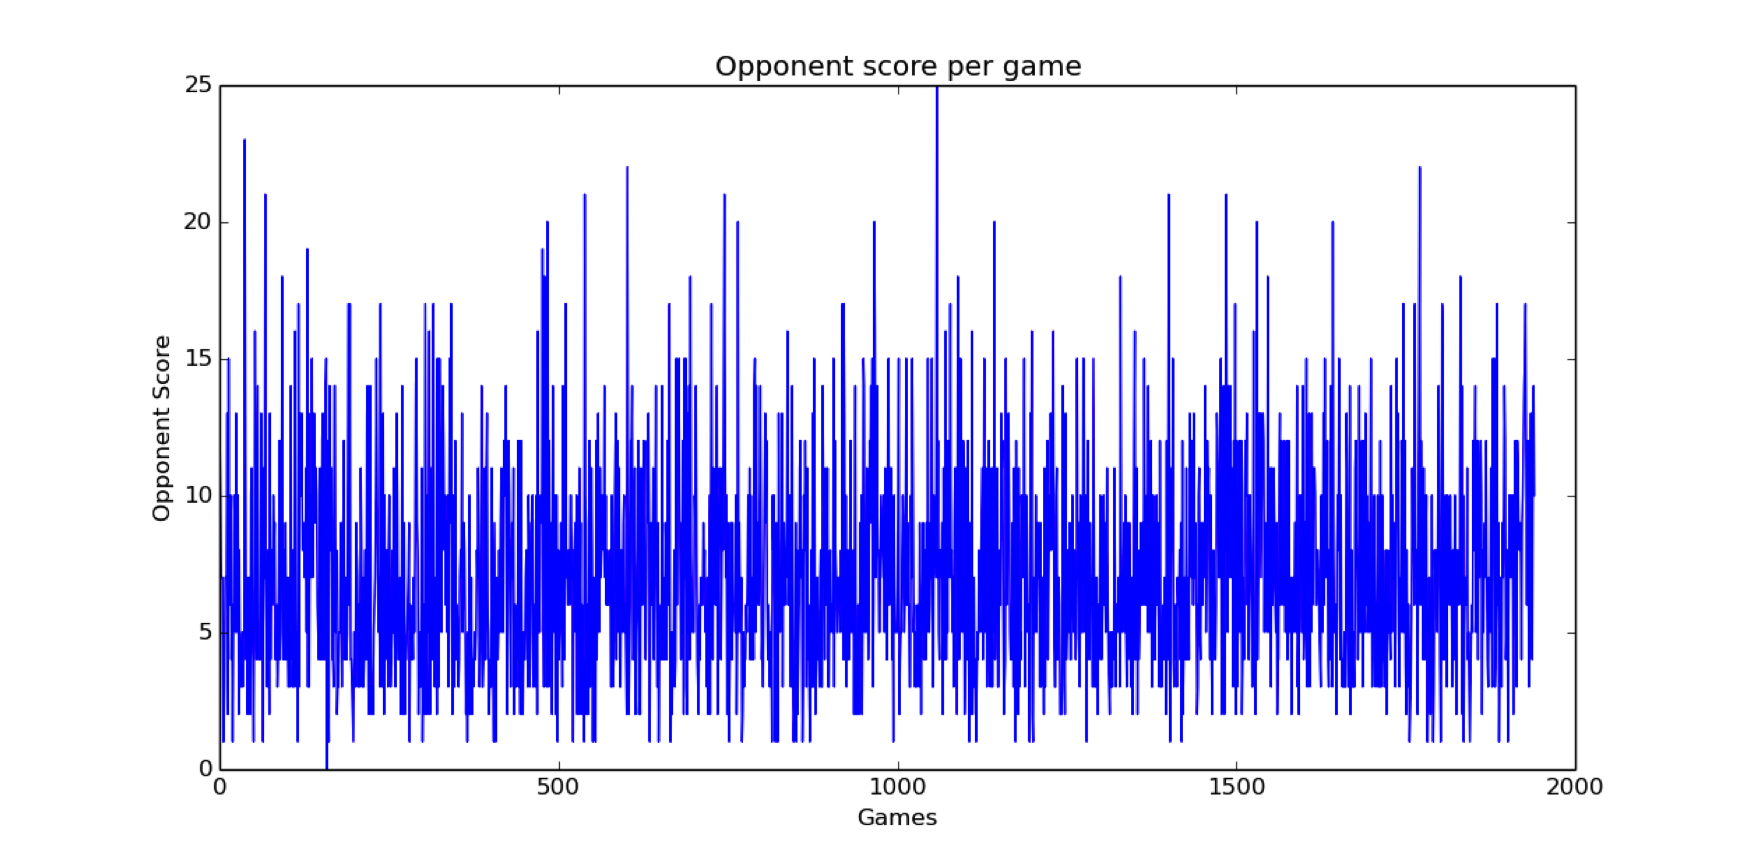
\includegraphics[scale=0.5]{training_score.png}
\caption{Opponent (GnuGo) score per game on a 7 $\times$ 7 board. The network was provided with a 7 layer input and consisted of 5 convolution layers}
\label{fig:score}
\end{figure}

\subsection*{Analysis}

\textcolor{red}{AM: need some analysis on why it didn't work... could possibly migrate this into the Future Work section instead.}